% 2015 年陕西卷（文史类）第 20 题：椭圆与过定点的弦（依固定扫描页重绘，只画拓扑与标号，不按比例）
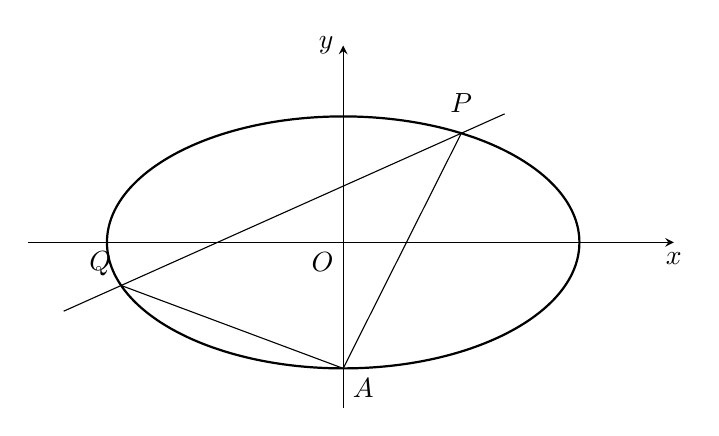
\begin{tikzpicture}[>=stealth,scale=1.0]
  % 坐标轴
  \draw[->] (-4.0,0)--(4.2,0) node[below] {$x$};
  \draw[->] (0,-2.1)--(0,2.5) node[left] {$y$};
  \node[below left] at (0,0) {$O$};
  % 椭圆
  \draw[thick] (0,0) ellipse (3 and 1.6);
  % 点 P、Q 与弦 PQ
  \coordinate (P) at (1.5,1.386);
  \coordinate (Q) at (-2.82,-0.547);
  \coordinate (A) at (0,-1.6);
  \draw (2.05,1.632)--(-3.55,-0.874);
  \draw (A)--(P);
  \draw (A)--(Q);
  \node[above=4pt] at (P) {$P$};
  \node[above left] at (Q) {$Q$};
  \node[below right] at (A) {$A$};
\end{tikzpicture}
